\chapter{Architecture and implementation}

% we now have a design and abstractions --> demonstrated by implemented prototype application
% demonstrates: abstractions works (can be implemented, is reasonable), extensibility,

% technology - .net 8, asp.net minimal api, angular, xunit(liek unit tests from chap 1)
% selected orms - nhibernate, ef core, dapper - WHY (most used, micro/macro, different mappings)

% highlevel architecture overview with diagram
% each project description, purpose

% patterns used - wrappers=adapters, factories, visitors  -    REST API?
% parser -> IR -> builder - explained earlier, just a short reminder - for easy extesnibility

% concrete wrappers
% entities - roslyn
% nhibernate mapping - liqn to xml
% builder - stringbuilders
% ef core linq - csharpsyntaxtreewalker
% dapper sql builder - visitor

% app screenshot?

% tests - integration tests for each wrapper, some combined integration tests (no unit tests!)

% deployment - dotnet run locally, possibly show nginx setup?

% limitations - what was not implemented 
%3 orms, only one query direction (and the parser is simple because the parsing is complex), no trees, NO DATABASE CONNECTION, no auto content detection
% to improve: better FE, security? (no validation)
% future work - ?

% summary - prototype was implemented, sucessfully demonstrates that the abstraction works


Building on the designed abstraction and algorithms from previous chapters, a prototype application is developed to demonstrate the feasibility of the concepts. The application presents a simple graphical user interface in the form of a single-page website. The background application provides interface for communication, all translation logic along with integration tests. Internally, the application adheres to design patterns proposed in earlier chapters. It implements parsers constructing the intermediate representation, which builders subsequently translate to user-selected \acrshort{orm}.

The application currently supports three \acrshort{orm} frameworks - Dapper, NHibernate, and \acrshort{efcore}. Those were chosen for their criteria analyzed in Chapter \ref{chapter:ormcomparison}, mainly their popularity and variety in mapping and querying. Dapper represents macro ORMs, with its lack of mapping and support for only \acrshort{sql} queries. \acrshort{efcore} was chosen for its feature set, extensive \acrshort{linq} coverage, and attribute mapping. NHibernate completes this set with a unique mapping format in \acrshort{xml} files.

Figure \ref{fig:supported_directions} visualizes currently supported translation directions. Entity and mapping configurations are translatable between all the three \acrshort{orm}s. The tool can translate \acrshort{efcore}'s \acrshort{linq} queries into Dapper's \acrshort{sql}.

\begin{figure}[!htp]
  \centering
  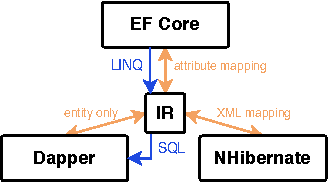
\includegraphics[scale=1.5]{thesis/img/thesis/06_supported_directions.drawio.pdf}
  \caption{Supported translation directions}
  \label{fig:supported_directions}
\end{figure}

\section{Application architecture}
The application is written in .NET 8 and is structured into multiple projects. In .NET, each project represents a distinct unit of compilation, functioning as an application module with explicitly defined dependencies. These projects are grouped within a .NET solution file, which can be managed and run through Visual Studio or any other \acrshort{ide}.\footnote{\url{https://learn.microsoft.com/en-us/visualstudio/ide/solutions-and-projects-in-visual-studio}} 

Figure \ref{fig:app_architecture} illustrates the application's decomposition. It consists of three project types. The first is an ASP.NET\footnote{\url{https://dotnet.microsoft.com/en-us/apps/aspnet}} web project used in the \texttt{ORMConvertorAPI} to provide data and translation interfaces to the frontend. Although the frontend is technically independent and runs within a browser, its static source files are served by this project. 
The second project type is a testing project based on the xUnit framework\footnote{\url{https://xunit.net/}}, used by the \texttt{Tests} project to perform integration tests. The remaining projects belong to the third category, basic C\# library projects, which are not executable and can only be utilized through references within executable projects.

\begin{figure}[!htp]
  \centering
  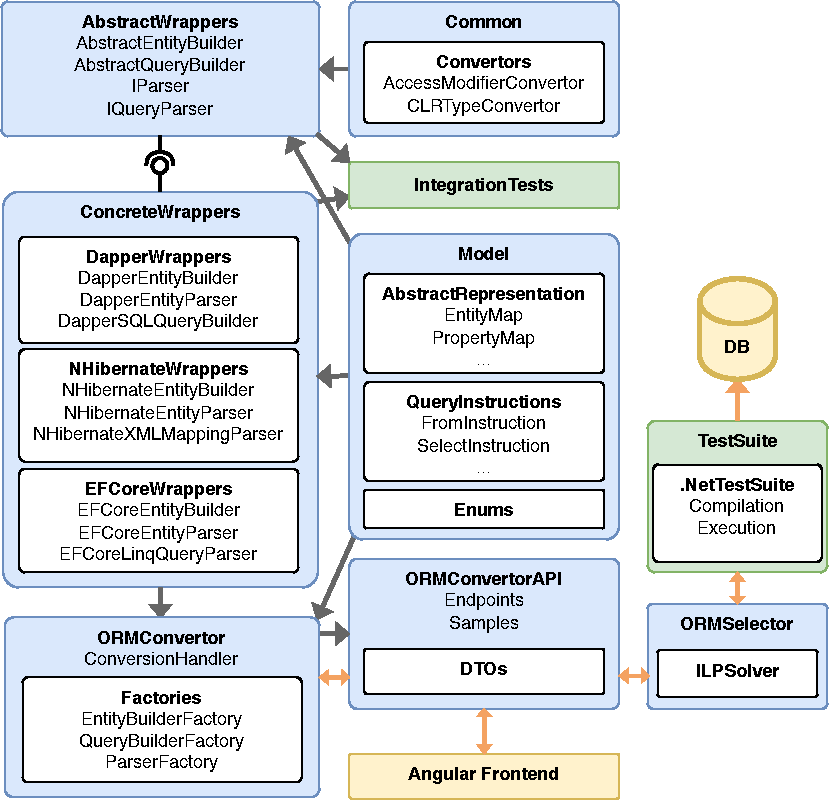
\includegraphics[scale=1]{thesis/img/thesis/06_architecture.drawio.pdf}
  \caption{Application architecture}
  \label{fig:app_architecture}
\end{figure}

\texttt{Model} is a central project containing domain models. It houses models for entity mapping intermediate representation designed in Chapter \ref{chapter:entity_translation} as well as immutable records representing instructions for queries from Chapter \ref{chapter:query_translation}. In addition, it has enumerations and other objects the application depends on. The project is referenced by almost all others as it is essential to application function.

\texttt{AbstractWrappers} defines interfaces for builders and parsers. As builders share some common functionality, they are declared as \textit{abstract} classes with some implemented methods. Parsers only declare an interface without any implementation. Concrete wrappers are then implemented in \texttt{ConcreteWrappers} project folder. Each ORM has its own project to isolate them and decouple dependencies.

The main translation algorithm is defined in \texttt{ORMConvertor} project in the \texttt{ConversionHandler} class. The class is responsible for receiving source \acrshort{orm} inputs, orchestrating appropriate parsers and builders, and returning correct output. \texttt{ConversionHandler} does not work with specific implementations, it only accesses them through interfaces. Factories are responsible for returning the correct wrappers and instantiating them. It is a direct implementation of Algorithm~\ref{alg:translation_alg}.

\section{Parser and builder wrappers}%just Wrappers?
Each wrapper --- either a parser or builder --- effectively serves as an adapter, translating between the specific interface of an \acrshort{orm} and the intermediate representation. Their function aligns with the \textit{adapter} pattern, enabling interoperability between otherwise incompatible representations.

Entity parsers for each framework follow a similar approach, leveraging the Roslyn syntax analyzer to extract class information. The Dapper parser handles only entity structure, while the \acrshort{efcore} parser also interprets attribute-based mapping. NHibernate employs two separate parsers: one mirrors the behaviour of the Dapper parser by processing only the entity, while the other parses the \acrshort{xml} mapping using \acrshort{linq} to \acrshort{xml}.

Currently, only parsing of \acrshort{efcore} \acrshort{linq} queries is supported. Due to the flexibility of \acrshort{linq} --- in method order and lambda expressions --- parsing is fairly complex. The implementation extends \texttt{CSharpSyntaxTree}, overriding the \texttt{Visit} method to analyze method call expressions. 

Entity builders follow an identical strategy, populating string templates and collecting the final structure in \texttt{StringBuilder}. The NHibernate builder separately constructs the entity class and  its corresponding \acrshort{xml} mapping.

For queries, only the Dapper \acrshort{sql} builder is implemented. It uses \texttt{StringBuilder} to sequentially assemble query components, while a dedicated visitor class handles concrete syntax generation.

% deployment + testing + github pipeline
% user interface

\begin{figure}[!htp]
  \centering
  \fbox{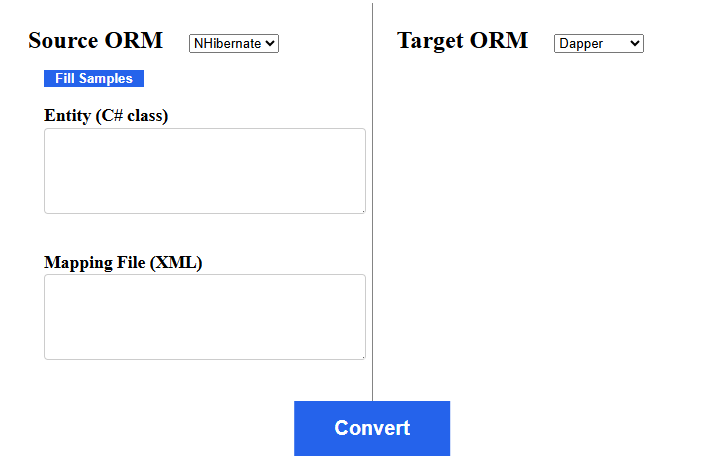
\includegraphics[scale=1]{thesis/img/thesis/06_app_ui.png}}
  \caption{Tool interface}
  \label{fig:tool_interface}
\end{figure}

\begin{landscape}
\begin{figure}[!htp]
  \centering
  \fbox{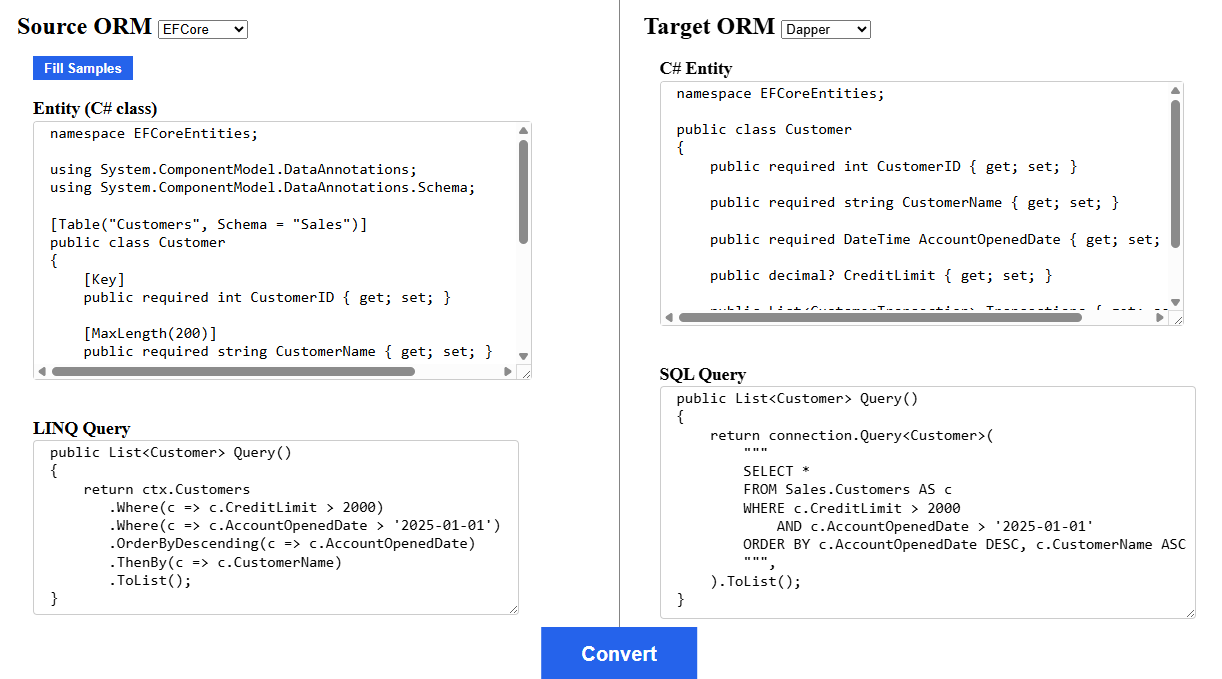
\includegraphics[width=0.9\textwidth]{thesis/img/thesis/06_app_ui_translated.png}}
  \caption{Tool interface - translation from \acrshort{efcore} to Dapper}
  \label{fig:tool_interface_translated}
\end{figure}
\end{landscape}